\documentclass[10pt,a4paper]{article}
\usepackage[utf8]{inputenc}
\usepackage{amsmath}
\usepackage{amsfonts}
\usepackage{amssymb}
\usepackage{booktabs}
\usepackage{tikz}
\usepackage{adjustbox}
\usepackage{caption}  
\usepackage{multirow}
\usepackage{algorithm}
\usepackage[noend]{algpseudocode}
\usepackage{listings}
\usepackage{xcolor}
\usepackage{pgfopts}
\usepackage{xstring}


\usetikzlibrary{positioning,angles,quotes,calc,shapes.geometric}
\usetikzlibrary{chains,shapes.multipart}
\usetikzlibrary{shapes,calc,fit}
\usetikzlibrary{automata,positioning}


\lstset{
language=Java,
basicstyle=\small\ttfamily,			
keywordstyle=\color{blue},
commentstyle=\color{gray},			
stringstyle=\color{black},			
numbers=left,						
numberstyle=\tiny,					
stepnumber=1,						
breaklines=true						
}


\begin{document}



\section{Goal}




\section{Conceptual Model}

Let's start with the \textit{second} step of a typical discrete-event simulation: the \textbf{conceptual model} building. 

First of all our system represents a network of nodes to which some application, running in set of external mobile devices, send their tasks, called \textbf{jobs}, because of performance or energy saving reasons. 

Not all job sent to system are the same, in fact we make distinction between two types of task, denoted as \textbf{class 1 job} and \textbf{class two job}; differences betweens them are described in following sections. 

To minimize mean response time experienced by mobile device users, the system is been built as a "\textit{two-layer}" network in such a way that an arriving job is sent, if possible, firstly to the nearest node.

\begin{adjustbox}{center=\textwidth}
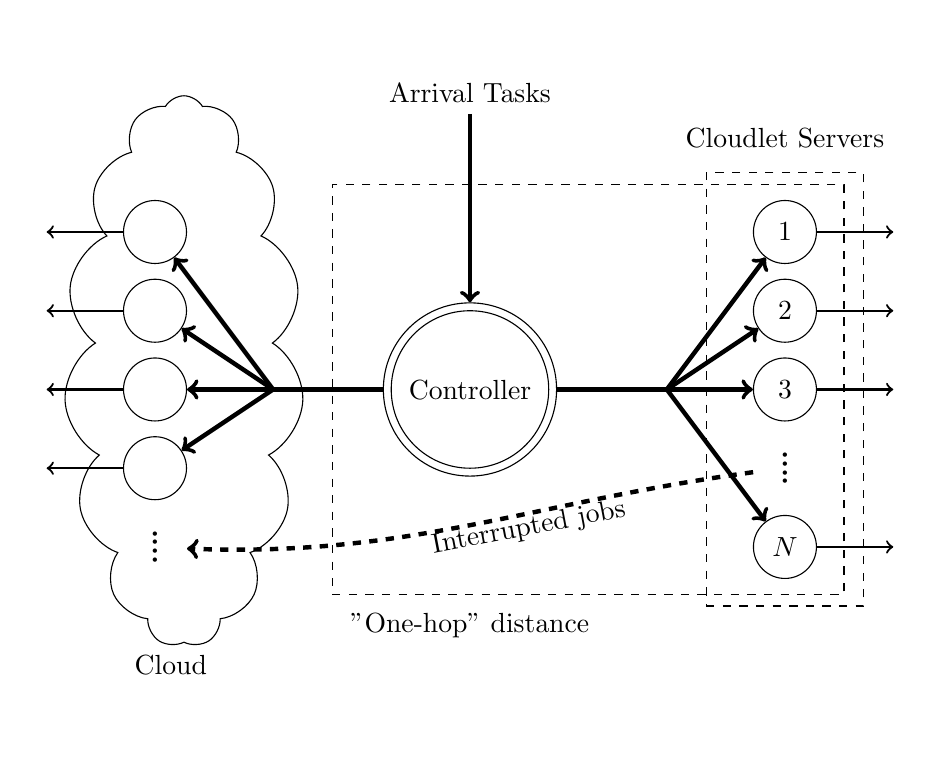
\begin{tikzpicture}


% Cloud

\node[circle, draw, minimum width = 0.8cm]        					   (CloudNode0) at (0,2) {};
\node[circle, draw, minimum width = 0.8cm, below of=CloudNode0]        (CloudNode1) {};
\node[circle, draw, minimum width = 0.8cm, below of=CloudNode1]        (CloudNode2) {};
\node[circle, draw, minimum width = 0.8cm, below of=CloudNode2]        (CloudNode3) {};
\node[circle, draw=white, minimum width = 0.8cm, below of=CloudNode3]  (CloudNode4) {\rotatebox{90}{\textbf{....}}};

\node[above of=CloudNode4, yshift=-2.5cm, xshift=0.2cm] (labellllllll) {Cloud};

\node[right of=CloudNode0, xshift=-2.5cm] (ExtCloudNode0) {};
\node[right of=CloudNode1, xshift=-2.5cm] (ExtCloudNode1) {};
\node[right of=CloudNode2, xshift=-2.5cm] (ExtCloudNode2) {};
\node[right of=CloudNode3, xshift=-2.5cm] (ExtCloudNode3) {};


\coordinate (cloudStartNode) at (1.5,0);

% Controller

\node[circle, draw, minimum width = 2.2cm]  (ControllerExternal) at (4,0) {};
\node[circle, draw, minimum width = 2cm]    (Controller2)        at (4,0) {Controller};

\coordinate (cloudletStartNode) at (6.5,0);

\coordinate (Start) at (4,3.5);

% Cloudlet

\node[circle, draw, minimum width = 0.8cm, left of=ControllerExternal, xshift=5cm, yshift=2cm]       (CloudletNode0) {$1$};
\node[circle, draw, minimum width = 0.8cm, below of=CloudletNode0]           (CloudletNode1) {$2$};
\node[circle, draw, minimum width = 0.8cm, below of=CloudletNode1]           (CloudletNode2) {$3$};
\node[circle, draw=white, minimum width = 0.8cm, below of=CloudletNode2]     (CloudletNode3) {\rotatebox{90}{\textbf{....}}};
\node[circle, draw, minimum width = 0.8cm, below of=CloudletNode3] (CloudletNode4) {$N$};

\node[rectangle, draw, dashed, minimum width =6.5cm, minimum height=5.2cm] (Cloudlet) at (5.5,0) {};
\node[circle,below of=Cloudlet, yshift=-2cm, xshift=-1.5cm] (label1) {"One-hop" distance};

\node[left of=CloudletNode0, xshift=2.5cm] (ExtCloudletNode0) {};
\node[left of=CloudletNode1, xshift=2.5cm] (ExtCloudletNode1) {};
\node[left of=CloudletNode2, xshift=2.5cm] (ExtCloudletNode2) {};
\node[left of=CloudletNode4, xshift=2.5cm] (ExtCloudletNode3) {};

\node[rectangle, draw, dashed, minimum width =2cm, minimum height=5.5cm, right of=CloudletNode2, xshift=-1cm] (CloudletFrame) {};
\node[circle,above of=CloudletFrame, yshift=2.2cm] (label1) {Cloudlet Servers};

% Cloudlet Rows...

\draw[ultra thick,-] (ControllerExternal) -- (cloudletStartNode);
\draw[ultra thick,->] (cloudletStartNode) -- (CloudletNode0);
\draw[ultra thick,->] (cloudletStartNode) -- (CloudletNode1);
\draw[ultra thick,->] (cloudletStartNode) -- (CloudletNode2);
\draw[ultra thick,->] (cloudletStartNode) -- (CloudletNode4);

% Cloud Rows...

\draw[ultra thick,-] (ControllerExternal) -- (cloudStartNode);
\draw[ultra thick,->] (cloudStartNode) -- (CloudNode0);
\draw[ultra thick,->] (cloudStartNode) -- (CloudNode1);
\draw[ultra thick,->] (cloudStartNode) -- (CloudNode2);
\draw[ultra thick,->] (cloudStartNode) -- (CloudNode3);

% Out from cloudlet nodes

\draw[thick,->] (CloudletNode0) -- (ExtCloudletNode0);
\draw[thick,->] (CloudletNode1) -- (ExtCloudletNode1);
\draw[thick,->] (CloudletNode2) -- (ExtCloudletNode2);
\draw[thick,->] (CloudletNode4) -- (ExtCloudletNode3);

% Out from cloud nodes

\draw[thick,->] (CloudNode0) -- (ExtCloudNode0);
\draw[thick,->] (CloudNode1) -- (ExtCloudNode1);
\draw[thick,->] (CloudNode2) -- (ExtCloudNode2);
\draw[thick,->] (CloudNode3) -- (ExtCloudNode3);
 
% START

\draw[ultra thick,->] (Start) node[above] {Arrival Tasks} -- (ControllerExternal) ;

\node [cloud, right of=CloudNode3, xshift=-18, yshift=35, draw,cloud puffs=15,cloud puff arc=120, aspect=3, minimum width =2.5cm, minimum height=7cm, inner ysep=1em] (cloudcc) {};

\path (CloudletNode3) edge[->,dashed,ultra thick, bend left, out=0, in=170] node [left] [sloped, yshift=-5,xshift=60] {Interrupted jobs} (CloudNode4);

\end{tikzpicture}
\end{adjustbox}



To be more precise, our system is made up of a set of nodes described below:

\begin{description}
\item[Cloudlet] It represents an \textit{edge cloud server} which, in addition to being located at "\textit{one-hop}" distance from mobile devices users, and therefore nearest to them, is able to guarantee absence of interferences among tasks allocated to it as long as their number does not exceed a given threshold $N$. From our conceptual model point of view, cloudlet represents a \textbf{fixed-capacity multi-server service node with any queue}.

Its capacity, that is the maximum possible number of jobs in it, is fixed to $N$

\item[Cloud] It represents a \textit{remote cloud server} which, although it \textbf{suffers for greater network delay}, due of its high distance from mobile devices, has virtually \textbf{unlimited resources} so that he can to process any number of tasks allocated to it. Consequently we had modelled this subsystem as an \textbf{unlimited-capacity multi-server service node with any queue}.

Being made up of an unlimited number of servers, its capacity is also unlimited.

\item[Controller] It represent the entry point of our system because all task are sent to it from outside in order to decide about whether an arrived job should be sent to the cloudlet or the cloud according to a given access control algorithm.

It is located on cloudlet and has the capability to precess each arriving job \textbf{instantaneously}. So that it is modelled simply as \textbf{single-server service node with no queue}. 

\end{description}

\begin{algorithm}

\caption{}\label{alg:accessControlAlgorithm1}

\begin{algorithmic}[1]

\Function{accessControlFunction}{$\textit{arrivalJob}$}

\If {$(n_1 + n_2=N)$}
	\State Send $\textit{arrivalJob}$ on the cloud.
\Else 	
 	\State Send $\textit{arrivalJob}$ on the cloudlet.
\EndIf

\EndFunction

\end{algorithmic}
\end{algorithm}

At this point, in order to properly define our conceptual model, we need to specify \textit{state variables} of our system. 
Due to access control algorithms characteristics, described below, we have decided to represent the state of our system as an ordered pair $(n_1, n_2)$ where $n_1$ represents the number of class one job while $n_2$ the number of class two job both contained in cloudlet. Consequently we have decided to just ignore type and number of jobs contained in cloud node because not relevant in any access control algorithms and negligible for goal of our study. 

A this point we can observe access control algorithms used by controller to make decisions which are fully described by their pseudo-code shown in Algorithm \ref{alg:accessControlAlgorithm1} and Algorithm \ref{alg:accessControlAlgorithm2}. 

Observe that to make its decision controller node can use only one access control algorithm at a time. 

Note that Algorithm \ref{alg:accessControlAlgorithm2} use a further threshold variable to make its decision denoted by $S$ which is less or equal than $N$. Remember that when a class 2 job is interrupted and sent on the cloud, a \textbf{ setup time} has to be considered to restart the task on the cloud. 

\begin{algorithm}[h]
\caption{}\label{alg:accessControlAlgorithm2}
\begin{algorithmic}[h!]

\Function{accessControlFunction}{$\textit{arrivalJob}$}

\If {$(\textit{arrivalJob.isClassOne})$}


\If {$n_1 = N$}
	\State Send $\textit{arrivalJob}$ on the cloud.

\ElsIf{$n_1 + n_2 \leq S $}
	\State Send $\textit{arrivalJob}$ on the cloudlet.
\ElsIf{$ n_2 \geq 0 $}
	\State Interrupt a class 2 job currently running on cloudlet.
	\State Send interrupted job to cloud.
	\State Send $\textit{arrivalJob}$ on the cloudlet.
\Else 	
 	\State Send $\textit{arrivalJob}$ on the cloudlet.
\EndIf



\Else 

\If {$(n_1 + n_2 \geq S)$}
	\State Send $\textit{arrivalJob}$ on the cloud.
\Else 	
 	\State Send $\textit{arrivalJob}$ on the cloudlet.
\EndIf

\EndIf

\EndFunction

\end{algorithmic}
\end{algorithm}

















\clearpage
\newpage
\section{Specification  Model}

In this section we will provide a \textit{specification model} of our system in which we will turn all system's states into a collection of mathematical variables together with equations and logic describing how the state variables are interrelated including algorithms for computing their interaction and evolution in time.\footnote{Lawrence M. Leemis, Stephen K. Park, \textit{Discrete-Event Simulation: A First Course} (Pearson; 1 edition January 6, 2006), 186}

\subsection{System's variables}

In order to properly describe all system's state variables, we need to introduce some mathematical notations.

$\tau \in (t_0, t)$ denotes a time's instant of our system simulation clock where $t_0$ and $t$ represent respectively \textit{start moment} and \textit{final moment} of our simulation; we will use also $c \in \lbrace 1,2 \rbrace = C$, representing the class to which a job belongs, and $x \in \lbrace cloudlet,cloud,global \rbrace = X$, used, instead, to refer to a specific system's node, or to whole system when $x = global$, where a job is running.

At this point we can introduce all mathematical variables used in our model:

\begin{table}[h!]
    \centering
    \small
    \begin{tabular}{rcl}
       
      $n_x^{(c)}(\tau)$ & $ = $ & Number of class $c$ jobs currently running at $x$ system's node at time $\tau$ \\
      $d_x^{(c)}(\tau)$ & $ = $ & Number of class $c$ departed jobs from node $x$ at time $\tau$ \\
      $s_{x,i}^{(c)}$ & $ = $ & Service time of class $c$ job $i$ served on $x$ node   \\
      $i_{cloudlet}^{(2)}$ & $ = $ & Number of class 2 interrupted job which were running on cloudlet node\\
          
    \end{tabular}
\end{table}

Is $n_x^{(c)}$ the number of class $c$ jobs running on node $x$. We define the \textbf{state} of our system as follow:

\begin{equation}
\omega = (\omega_{cloudlet},\omega_{cloud})
\end{equation}

In this context, $\omega_{cloudlet}$ and $\omega_{cloud}$ are the states of cloudlet and cloud node respectively. Specifically:

\begin{equation}
\begin{array} {rcl} 
\omega_{cloudlet} & = & (n_{cloudlet}^{(1)},n_{cloudlet}^{(2)}) \\
\omega_{cloud} & = & (n_{cloud}^{(1)},n_{cloud}^{(2)}) \\
\end{array}
\end{equation}

Thus:

\begin{equation}
\begin{array} {rcl} 
\omega = ((n_{cloudlet}^{(1)},n_{cloudlet}^{(2)}),(n_{cloud}^{(1)},n_{cloud}^{(2)})
\end{array}
\end{equation}

At this point we can show some equations describing constrains or relations among these variables.

Obliviously is true that:

\begin{equation}
\begin{array} {lr} 
\displaystyle n_{global}^{(c)}(\tau) = \sum_{x \in X \setminus \lbrace global \rbrace } n_x^{(c)}(\tau) & \forall c \in C, \forall \tau \in (t_0, t)
\end{array}
\end{equation}

\begin{equation}
\begin{array} {lr} 
\displaystyle d_{global}^{(c)}(\tau) = \sum_{x \in X \setminus \lbrace global \rbrace } d_x^{(c)}(\tau) & \forall c \in C, \forall \tau \in (t_0, t)
\end{array}
\end{equation}

If our system is based on Algorithm \ref{alg:accessControlAlgorithm1}, is true that:

\begin{equation}
\begin{array} {lr} 
\displaystyle \sum_{c \in C} n_{cloudlet}^{(c)}(\tau) \leq N & \forall \tau \in (t_0, t)
\end{array}
\end{equation}

When, instead, our system is using Algorithm \ref{alg:accessControlAlgorithm2}, is verified that:

\begin{equation}
\begin{array} {rccr} 
\displaystyle \sum_{c \in C} n_{cloudlet}^{(c)}(\tau) \leq S & \Leftrightarrow & n_{cloudlet}^{(2)}(\tau) > 0 & \forall \tau \in (t_0, t) \\
n_{cloudlet}^{(1)}(\tau) \leq N & \Leftrightarrow & n_{cloudlet}^{(2)}(\tau) = 0 & \forall \tau \in (t_0, t)
\end{array}
\end{equation}

\subsection{Statistics computing}

During this subsection we will describe how we can compute all system's statistics which we need using mathematical notation explained before.

\paragraph{Time-averaged population}

In order to compute $E[N_x](c)$, that is the \textit{time-averaged number of $c$ class jobs} in $x$ system's node, we can do as follows:\footnote{\textit{Ibid.}, 19}

\begin{equation}
\begin{array} {rclr} 
E[N_x](c) & = & \displaystyle  \dfrac{1}{t-t_0}\int_{t_0}^t n_x^{(c)}(\tau)d\tau & \forall c \in C, \forall x \in X
\end{array}
\end{equation}

To calculate instead $E[N_x]$, \textit{not-class-based time-averaged number of jobs} running in a $x$ system's node, we can proceed as shown below:

\begin{equation}
\begin{array} {rclr} 
E[N_x] & = & \displaystyle  \dfrac{1}{t-t_0} \cdot \int_{t_0}^t \left( n_x^{(1)}(\tau) + n_x^{(2)}(\tau) \right) d\tau \\\\
	   & = & \displaystyle  \dfrac{1}{t-t_0} \cdot \int_{t_0}^t n_x^{(1)}(\tau)d\tau + \dfrac{1}{t-t_0} \cdot \int_{t_0}^t n_x^{(2)}(\tau)d\tau \\\\
	   & = & E[N_x](1) + E[N_x](2) \\\\
	   & = & \displaystyle  \sum_{c \in C} E[N_x](c) & \forall x \in X
\end{array}
\end{equation}

\paragraph{Time-average response time}

Are $E[S_x](c)$ and $E[T_x](c)$ respectively the \textit{time-averaged service time of class $c$ jobs} and the \textit{per-class time-averaged response time} experienced by a class $c$ job in $x$ system's node. 

Since our system hasn't queues, there is no waiting time or delay experienced by jobs in our system, therefore result that $E[S_x](c) = E[T_x](c)$.
Said that, we just have to show how to compute $E[S_x](c)$:\footnote{\textit{Ibid.}, 17}

\begin{equation}
\begin{array} {rccccr} 
E[T_x](c) & = & E[S_x](c) & = & \displaystyle \dfrac{1}{d_x^{(c)}(t)} \cdot \sum_{i = 0}^{d_x^{(c)}(t)} s_{x,i}^{(c)} & \forall c \in C, \forall x \in X \\
\end{array}
\end{equation}

If we aren't interested about per-class metrics, we can compute $E[S_x]$ and $E[T_x]$, respectively \textit{time-averaged service time} and the \textit{time-averaged response time} experienced by any class jobs in a $x$ system's node, as follows:

\begin{equation}
\begin{array} {rccccr} 
E[T_x] & = & E[S_x] & = & \displaystyle \dfrac{1}{d_x^{(1)}(t) + d_x^{(2)}(t)} \cdot \left( \sum_{i = 0}^{d_x^{(1)}(t)} s_{x,i}^{(1)} + \sum_{i = 0}^{d_x^{(2)}(t)} s_{x,i}^{(2)} \right) & \forall x \in X \\
\end{array}
\end{equation}

\paragraph{Throughput}

\textit{Per-class system's node throughput}, denoted with $X_x(c)$, is the rate of per-class $c$ completions at $x$ system's node, while \textit{system's node throughput}, indicated with $X_x$, is the rate of any class job completions at $x$ system's node\footnote{Mor Harchol-Balter, \textit{Performance Modeling and Design of Computer Systems} (Carnegie Mellon University, Pennsylvania 2013), 18}. 

Generally the throughput is the ratio between the total number of jobs completed and observation time\footnote{\textit{Ibid.}}, therefore aforesaid metrics are simply computable as follows:

\begin{equation}
\begin{array} {rccr} 
X_x(c) & = & \displaystyle \dfrac{d_x^{(c)}(t)}{t} & \forall c \in C, \forall x \in X \\
\end{array}
\end{equation}

\begin{equation}
\begin{array} {rccr} 
X_x & = & \displaystyle \dfrac{d_x^{(1)} + d_x^{(2)}(t)}{t} & \forall x \in X \\
V_V++
\end{array}
\end{equation}

\subsection{System's events and assumptions}

Let's look to all possible \textit{events} which can occurs during our simulation. 

Since by definition any event is an occurrence that may change the state of the system\footnote{Lawrence M. Leemis, Stephen K. Park, \textit{Discrete-Event Simulation: A First Course} (Pearson; 1 edition January 6, 2006), 187}, obviously our system's state variables can change only when an event occurs.

All event capable to alter our system's state are reported in table \ref{table:SystemEvents}.

Finally, to complete to turn out our conceptual model into a proper specification model, we have to make additional assumptions which we have reported below:

\begin{itemize}
\item Although initial state variables can have any non-negative integer value\footnote{\textit{Ibid.} 190}, we have choosen, as common, to set $n_x^{(j)}(0) = 0$ and $d_x^{(j)}(0) = 0$ setting, in this way, initial system status as \textit{idle}. 

\item As a consequence of the previous point, first event must be either a \textit{Class 1 Job arrival} or a
\textit{Class 2 Job arrival} both on controller node.

\item Terminal state is also idle. Rather than specifying the number of jobs processed, our stopping criteria has been specified in terms of a time $\tau$ beyond which no new jobs can arrive. This assumption effectively closes the door at time $\tau$ but allows the system to continue operation until all jobs have been completely served. 

Therefore, the last event must be either a class 1 or class 2 job completion.
\end{itemize}



\begin{table}[h!]
    \caption{System's events}
    \begin{adjustbox}{center=\textwidth}
    \label{table:SystemEvents}
     \begin{tabular}{c|c|p{2.5cm}}

      \toprule
      \textbf{Event name that occurred at time $\tau$} & \textbf{Event's place} & \textbf{Event's effects} \\
      \midrule
      
      \multirow{3}{*}{Class 1 job arrival} & Cloudlet & $n_{\text{cloudlet}}^{(1)}(\tau)\texttt{++}$ \\ \cline{2-3} 
      & Cloud & $n_{\text{cloud}}^{(1)}(\tau)\texttt{++}$ \\ \cline{2-3} 
      & Controller & $n_{\text{global}}^{(1)}(\tau)\texttt{++}$ \\ 
       
      \hline
       
      \multirow{3}{*}{Class 2 job arrival} & Cloudlet & $n_{\text{cloudlet}}^{(2)}(\tau)\texttt{++}$ \\ \cline{2-3} 
      & Cloud & $n_{\text{cloud}}^{(2)}(\tau)\texttt{++}$ \\ \cline{2-3} 
      & Controller & $n_{\text{global}}^{(2)}(\tau)\texttt{++}$ \\ 
    
	  \hline
       
      \multirow{8}{*}{Class 1 job departure} & \multirow{4}{*}{Cloudlet} & $n_{\text{cloudlet}}^{(1)}(\tau)\texttt{--}$ \newline $n_{\text{global}}^{(1)}(\tau)\texttt{--}$ \newline $d_{\text{cloudlet}}^{(1)}(\tau)\texttt{++}$ \newline $d_{\text{global}}^{(1)}(\tau)\texttt{++}$ \\ \cline{2-3} 
      & \multirow{4}{*}{Cloud} & $n_{\text{cloud}}^{(1)}(\tau)\texttt{--}$ \newline $n_{\text{global}}^{(1)}(\tau)\texttt{--}$ \newline $d_{\text{cloud}}^{(1)}(\tau)\texttt{++}$ \newline $d_{\text{global}}^{(1)}(\tau)\texttt{++}$ \\ \cline{2-3} 
 
 		\hline
       
      \multirow{8}{*}{Class 2 job departure} & \multirow{4}{*}{Cloudlet} & $n_{\text{cloudlet}}^{(2)}(\tau)\texttt{--}$ \newline $n_{\text{global}}^{(2)}(\tau)\texttt{--}$ \newline $d_{\text{cloudlet}}^{(2)}(\tau)\texttt{++}$ \newline $d_{\text{global}}^{(2)}(\tau)\texttt{++}$ \\ \cline{2-3} 
      & \multirow{4}{*}{Cloud} & $n_{\text{cloud}}^{(2)}(\tau)\texttt{--}$ \newline $n_{\text{global}}^{(2)}(\tau)\texttt{--}$ \newline $d_{\text{cloud}}^{(2)}(\tau)\texttt{++}$ \newline $d_{\text{global}}^{(2)}(\tau)\texttt{++}$ \\
 
      \bottomrule


    \end{tabular}
    \end{adjustbox}
\end{table}





\newpage
\section{Computational Model}

Let's start now description about our system \textit{computational model} in which, as known, system's states exist as a collection of data structure, classes and variables that collectively characterize the system and are systematically updated as simulated time evolves.

\begin{figure}[H]
\includegraphics[width=\textwidth]{ClassDiagram}
\centering
\caption{Class diagram showing main classes and methods only.}

\label{fig:EventClassDiagram}

\end{figure}


\subsection{Events implementation}

In order to properly build discrete-event simulation models using \textit{next-event} approach we need to understand how all system's events, seen in previous section, are implemented and managed.

As shown in figure \ref{fig:EventClassDiagram}, a \textit{generic} system's event has been implemented and represented using an \textit{abstract} Java class called \texttt{SimulationEvent} which has two main features:

\begin{itemize}
\item Has only one \texttt{double} type field, called \texttt{StartTime}, used to hold instant of time according to which an event occurs.
\item Defines interfaces of two very important methods, used by the next-event simulation algorithm implemented in \texttt{ComputationalModel} class, which we will fully describe in next section, called \texttt{perform()}, used to update system's state variables when an event occurs, and \texttt{schedule\-Following\-Event()}, which is used, instead, to inserts into an \textit{event list} events that follows the current one.
\end{itemize}

Obviously exact methods behaviour depends strictly by which class implements it, however is very important to point out that \texttt{SimulationEvent} class does \textit{not} represent system-specific events; in fact, to ensure low coupling and high cohesion among classes, \texttt{ComputationalModel} doesn't need, and doesn't have to, know any specific system event information. 
 
System-specific event are instead represented by instances of \texttt{SystemEvent} class, partially shown in listing \ref{code:SystemEvent}. Any \texttt{SystemEvent} instance, knowing knowledge about which system's component is involved during an event occurrence, can, implementing \texttt{perform()} method, update state variable of that component taking into account its current state, without altering others parts of system. To be more precise, as you can see from the class diagram shown in figure \ref{fig:EventClassDiagram}, \texttt{perform()} method implementation is provided by \texttt{SystemEvent} subclasses which provide own very specific methods implementation in order to properly simulate effects of each specific system described before.

In this way, taking advantage of polymorphism pattern, every \texttt{SystemEvent} subtype instance can update properly each system's component, including whole system state, while \texttt{ComputationalModel} instance, which actively execute next-event simulation algorithm calling method implemented by them, ignores all specific information about our system.

To reduce further coupling between classes during \texttt{SystemEvent} object instantiation, a sort of factory method pattern, based on Java reflection ability, is used.

\begin{lstlisting}[frame=lines, caption={\texttt{SimulationEvent} class implementation.}, label={code:SystemEvent}]
public abstract class SystemEvent extends SimulationEvent {

    protected SystemComponent systemComponent;

    public void setSystemComponent(SystemComponent systemComponent) {
        this.systemComponent = systemComponent;
    }

    public SystemComponent getSystemComponent() {
        return systemComponent;
    }
    ...
\end{lstlisting}

\subsection{Event list}

As known, an \textit{event list}, also called \textit{calendar}, represents a data structure used to keep track of scheduled time of occurrence for the next possible event.

For reasons of efficiency, our event list is been implemented as a \textit{min-heap binary tree}, that is a \textit{priority queue} in which all events are ordered by time, in such a way that the most imminent event is found on the tree's root, providing $O(log_2(n))$ time for the en-queuing and dequeuing operation and constant time for root element retrieval.\footnote{Camil Demetrescu, Irene Finocchi, Giuseppe F. Italiano - \textit{Algorimti e strutture dati} - second edition, McGraw-Hill, pag. 200} 

Its implementation is already available in JDK through Java built-in class called \texttt{PriorityQueue$<$E$>$} which provides all method that we need.
However, in order to work properly, is required that a total ordering among all possible event exist. To provide it, we need all events instances implement an interface called \texttt{Comparable} providing an implementation, shown in listing \ref{code:compareTo}, of a method called \texttt{compareTo}.

Remember that \texttt{compareTo} method returns a negative integer, zero, or a positive integer if an  this object is less than, equal to, or greater than the specified object.\footnote{See \texttt{https://docs.oracle.com/en/java/javase/12/docs/api/java.base/java/lang/Comparable.html\#compareTo(T)}}


\begin{lstlisting}[frame=lines, caption={Snippet of \texttt{SimulationEvent} class implementation}, label={code:compareTo}]
@Override
public int compareTo(SimulationEvent o) {
	return Double.compare(this.startTime, o.startTime);
}
\end{lstlisting}

\subsection{Simulation clock}

As we know a \textit{simulation clock} is necessary to keep track of the current value of simulated time during simulation. 

In our system's implementation, our simulation clock is represented by a \texttt{SimulationClock} type instance, which partial implementation is reported in listing \ref{code:SimulationClock}. Simulation clock state is represented by two \texttt{double} type fields of which one, called \texttt{currentEventTime}, is used to holding current event simulated time value, while the second, called \texttt{nextEventTime}, is used to keep track of next event simulated time value.

From software architecture point of view, as you can see by code snippet shown below, believing that multiple \texttt{SimulationClock} instance are not necessary, that class is been implemented using \textit{singleton} pattern. 

\begin{lstlisting}[frame=lines, caption={\texttt{SimulationClock} class implementation.}, label={code:SimulationClock}]
public class SimulationClock {

    private static SimulationClock instance = null;

    private double currentEventTime;
    private double nextEventTime;

    private SimulationClock(){
    }

    public static SimulationClock getInstance() {
        if (instance == null)
            instance = new SimulationClock();
        return instance;
    }
    
    /* ... */
\end{lstlisting}


\subsection{Next-event simulation logic}

To execute a next-event simulation, we simply need to call a method, called \texttt{perform()}, using an instance of \texttt{ComputationalModel} class.
As shown in listing \ref{code:perform}, in that method has been implemented the algorithm \footnote{See Algorithm 5.1.1, pag. 189} used to perform our simulation, which consists of the following steps: 

\begin{description}
\item[Simulation initialization] As the phase name suggested, this step is performed to initialize system's state variables, including simulation clock and event list, inserting into them first possible events.

As you can see from code snippet, this task is performed calling \texttt{initialize\-Simulation()} method, which make a set of call to some abstract methods that have to be implemented by a concrete class which will describe next. 

\item[Process current event] Until event list is not empty (line 6), the most imminent possible event is extracted and removed from event list (line 8); then simulation clock is advanced to this event's scheduled time of occurrence (line 12) and finally system state is updated (line 14). 

\item[Schedule following event] Until a fixed simulation time $\tau$ in not exceeded, a new event is generated by current event and consequently placed into event list. Subsequently simulation clock instance field, used to holding time of occurrence of next possible event, is updated in order to compute some system metrics.

\item[Statistic update] While simulation advance from one event time to the next, calling an abstract method called \texttt{updateStatistics()}, all system's statistic metrics are updated.

\item[Simulation result generation and print] During this final step all data previously computed are elaborated using batch means approach and output data saved on file system.
\end{description}

\begin{lstlisting}[frame=lines, caption={Snippet of \texttt{perform} method}, label={code:perform}]
...
public void perform() {

        initializeSimulation();

        while (!this.simulationEventList.isEmpty()) {

            SimulationEvent actualEvent = this.simulationEventList.poll();

            if (actualEvent != null) {

                SimulationClock.getInstance().setCurrentEventTime(actualEvent.getStartTime());

                actualEvent.perform();
                actualEvent.scheduleFollowingEvent();

                SimulationEvent nextEvent = this.simulationEventList.peek();

                if (nextEvent != null)
                    SimulationClock.getInstance().setNextEventTime(nextEvent.getStartTime());
            }
            updateStatistics();
        }

        produceStatisticResultsThroughBatchMeansMethod();

        printSimulationResults();
    }
...
\end{lstlisting}


\subsection{System network implementation}

While a very generic queues network is represented by an instance of \texttt{ComputationalModel} class, our specific system is been modelled using \texttt{System} type instances which have very important responsibilities including:

A System type instance has many role including:

\begin{itemize}

\item Allocates \texttt{SystemComponent} type instances used to represent each system's nodes.

\item Initializes all instance fields representing a system variables of each system's node including simulated clock.

\item Updates event list for future events scheduling on each system's component. 

\end{itemize}

As we now 

\texttt{SystemComponent} class has key role during our simulation performing because:
\begin{itemize}

\item Has a set of fields used to keep track of component's variable states, like number of departed jobs or current jobs population, including those used to compute time-average statistics.

\item Provides a very important set of functions for status updating after event occurrences; for example, when a class one job arrives on a certain system's component, \texttt{updateStatusAfterClass1JobArrival()} method can be invoked in order to update the number of class one jobs actually present on that component.

\item Contains a set of method used to computed inter-arrival and service times, necessary for future event scheduling. Obviously each concrete \texttt{SystemComponent} instance has his own mean rates to compute those values.

\item Includes another set used instead to schedule future events after event occurrence, like a departure after an arrival. 

Is very important to precise that these methods are abstract and have to be implemented by each concrete implementations in order to reflect each component behaviour; In fact controller node doesn't need to schedule departure after an arrival because of his routing role.
\end{itemize}

All system's component, that is cloud, cloudlet and controller, are represented, obviously, by \texttt{Cloud}, \texttt{Cloudlet} and \texttt{Controller} classes each of which is a \texttt{SystemComponent} subclass; however we have used another subclass, called \texttt{GlobalNetwork}, in order to represent whole system keeping track of golabal state variables.

Observe that, \texttt{Controller} class is also an abstract class because required implementation of a method call \texttt{performRoutingAlgorithm()} used to perform the two required routing algorithms whenever an arrival occurs on controller node; those algorithms are provide by \texttt{ControllerUsingRoutingAlgorithm1} and \texttt{ControllerUsingRoutingAlgorithm2} classes. 

\subsection{Output analysis}

each statistic is associate to an TransientStatistics type instance.























\newpage
\section{Analytical solution}

In this last section we will develop an analytical solution to validate the results obtained previously through our simulations. 

\subsection{System based on access control Algorithm 1}
\begin{figure}
\caption{Access control algorithm 1 based cloudlet's CTMC.} \label{fig:ALG1-CloudletMarkovChain}
\begin{adjustbox}{center=\textwidth}
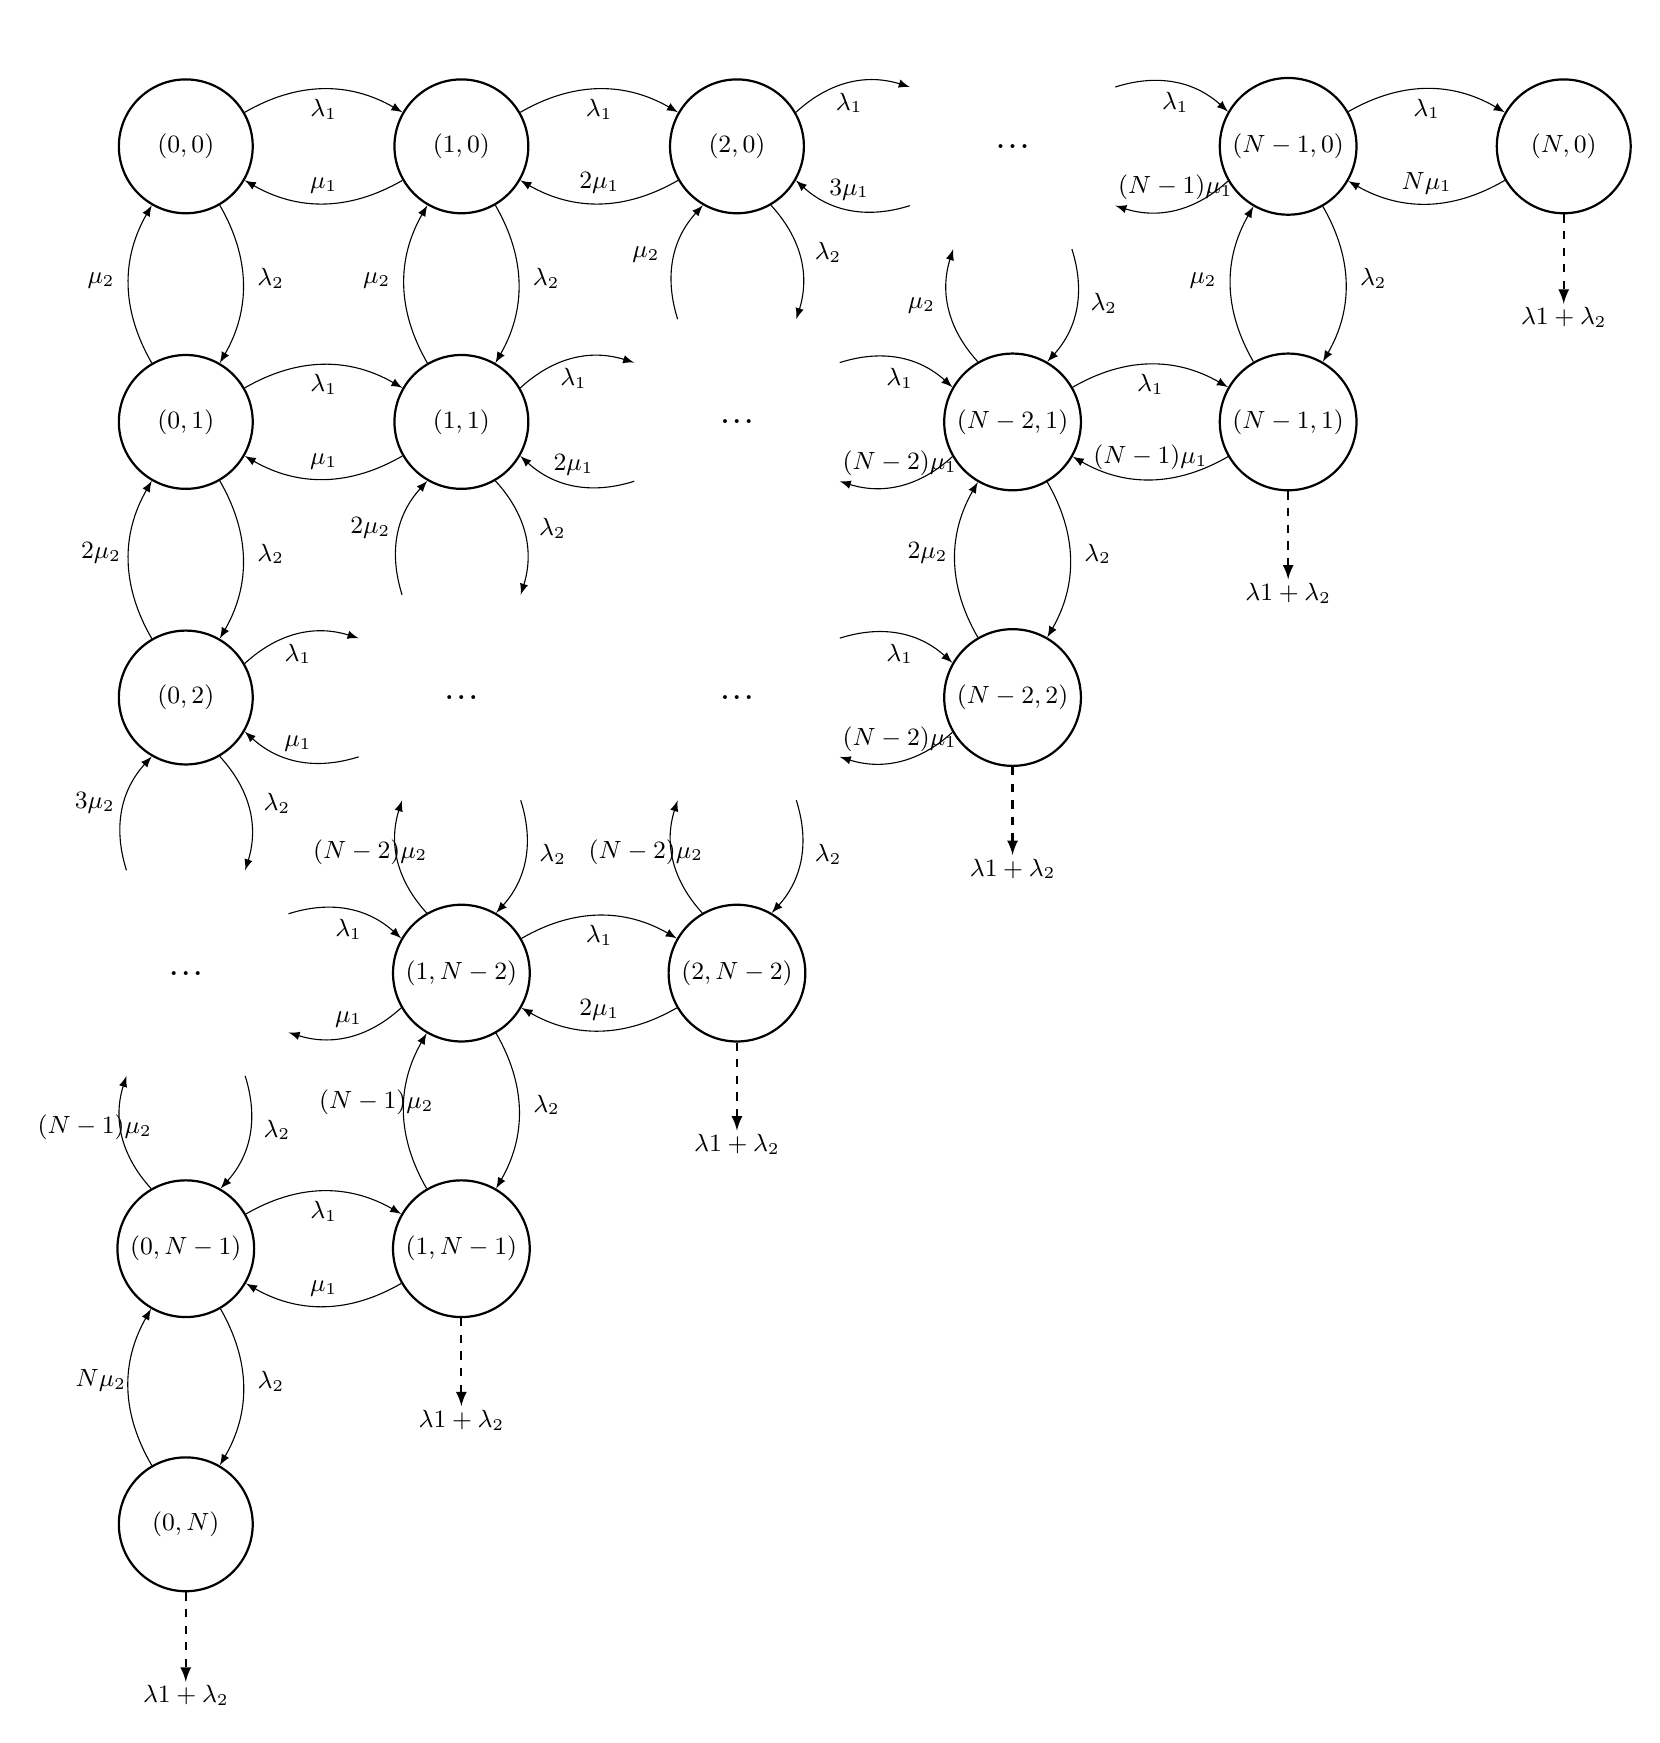
\begin{tikzpicture}[->,node distance=3.5cm,>=latex,font=\small, minimum width=1.7cm]

    \tikzstyle{round}=[thick,draw=black,circle]

    \node[round] 			    (00) {$(0,0)$};
    \node[round,right of=00]    (10) {$(1,0)$};
    \node[round,below of=00]    (01) {$(0,1)$};
    \node[round,below of=10]    (11) {$(1,1)$};
    \node[round,below of=01]    (02) {$(0,2)$};
    \node[round,right of=10]    (20) {$(2,0)$};
   
    \node[circle,draw=white,right of=20, minimum width = 3cm]    (A1) {\LARGE ...};
    \node[circle,draw=white,below of=02, minimum width = 3cm]    (A2) {\LARGE ...};
     
   	\node[round,right of=A1]    (N-1/0)  	{$(N-1,0)$};
   	\node[round,right of=N-1/0] (N0)	 	{$(N,0)$};
    \node[round,below of=N-1/0] (N-1/1)     {$(N-1,1)$};
    \node[round,left  of=N-1/1] (N-2/1)	{$(N-2,1)$};
    \node[round,below of=N-2/1] (N-2/2)	{$(N-2,2)$};
   
    \node[round,below of=A2]    (0/N-1)  	{$(0,N-1)$};
   	\node[round,below of=0/N-1] (0N)	 	{$(0,N)$};
    \node[round,right of=0/N-1] (1/N-1)     {$(1,N-1)$};
    \node[round,above of=1/N-1] (1/N-2)     {$(1,N-2)$};
    \node[round,right of=1/N-2] (2/N-2)	    {$(2,N-2)$};
    
    
    \node[circle,draw=white,left of=N-2/1,minimum width = 3cm]        (A3)     {\LARGE ...};
    \node[circle,draw=white,below of=11,minimum width = 3cm]          (A4)     {\LARGE ...};
    \node[circle,draw=white,above of=2/N-2,minimum width = 3cm]       (A5)     {\LARGE ...};
 
 	\draw[dashed,thick, ->] (N0) -- +(0,-2) node[yshift=-5]  {$\lambda1+\lambda_2$};
 	\draw[dashed,thick, ->] (N-1/1) -- +(0,-2) node[yshift=-5]  {$\lambda1+\lambda_2$};
 	\draw[dashed,thick, ->] (N-2/2) -- +(0,-2) node[yshift=-5]  {$\lambda1+\lambda_2$};
 	\draw[dashed,thick, ->] (2/N-2) -- +(0,-2) node[yshift=-5]  {$\lambda1+\lambda_2$};
 	\draw[dashed,thick, ->] (1/N-1) -- +(0,-2) node[yshift=-5]  {$\lambda1+\lambda_2$};
 	\draw[dashed,thick, ->] (0N) -- +(0,-2) node[yshift=-5]  {$\lambda1+\lambda_2$};
 
 	\path 
 	(00) 	edge[bend left,below]		node 					    {$\lambda_1$}		(10)
 		 	edge[bend left,above]       node [xshift=10,yshift=-5]  {$\lambda_2$} 		(01)
 	
 	(10) 	edge[bend left,above]       node 						{$\mu_1$} 			(00)
 		 	edge[bend left,below]		node 					    {$\lambda_1$}		(20)
 		 	edge[bend left,above]       node [xshift=10,yshift=-5]  {$\lambda_2$} 		(11)
 	
    (01) 	edge[bend left,above]       node [xshift=-10,yshift=-5] {$\mu_2$} 			(00)
   		 	edge[bend left,below]		node 					    {$\lambda_1$}		(11)
   	     	edge[bend left,above]       node [xshift=10,yshift=-5]  {$\lambda_2$} 		(02)
   
    (20) 	edge[bend left,above]       node 						{$2\mu_1$} 			(10)
    		edge[bend left,below]		node 					    {$\lambda_1$}		(A1)
    		edge[bend left,above]       node [xshift=10,yshift=-5]  {$\lambda_2$} 		(A3)
   		    
    (02) 	edge[bend left,above]       node [xshift=-10,yshift=-5] {$2\mu_2$} 			(01)
    		edge[bend left,above]       node [xshift=10,yshift=-5]  {$\lambda_2$} 		(A2)
    		edge[bend left,below]		node 					    {$\lambda_1$}		(A4)
   
    (11) 	edge[bend left,above]       node [xshift=-10,yshift=-5] {$\mu_2$} 			(10)
   		 	edge[bend left,above]       node 						{$\mu_1$} 			(01)
   		 	edge[bend left,below]		node 					    {$\lambda_1$}		(A3)
   		 	edge[bend left,above]       node [xshift=10,yshift=-5]  {$\lambda_2$} 		(A4)
   
   	(N0) 	edge[bend left,above]       node 						{$N\mu_1$} 			(N-1/0)
   
   	(N-1/0) edge[bend left,below]		node 					    {$\lambda_1$}		(N0)
   			edge[bend left,above]       node [xshift=10,yshift=-5]  {$\lambda_2$} 		(N-1/1)
   			edge[bend left,above]       node 						{$(N-1)\mu_1$} 			(A1)
   
    (N-1/1) edge[bend left,above]       node [xshift=-10,yshift=-5] {$\mu_2$} 			(N-1/0)
    		edge[bend left,above]       node 						{$(N-1)\mu_1$} 		(N-2/1)
    
    (N-2/1) edge[bend left,below]		node 					    {$\lambda_1$}		(N-1/1)
    		edge[bend left,above]       node [xshift=-10,yshift=-5] {$\mu_2$} 			(A1)
    		edge[bend left,above]       node 						{$(N-2)\mu_1$} 		(A3)
    		edge[bend left,above]       node [xshift=10,yshift=-5]  {$\lambda_2$} 		(N-2/2)
    		
    (N-2/2) edge[bend left,above]       node [xshift=-10,yshift=-5] {$2\mu_2$} 			(N-2/1)
    		edge[bend left,above]       node 						{$(N-2)\mu_1$} 		(A5)
    
    (0N) 	edge[bend left,above]       node [xshift=-10,yshift=-5]	{$N\mu_2$} 			(0/N-1)
   
   	(0/N-1) edge[bend left,below]		node 					    {$\lambda_1$}		(1/N-1)
   			edge[bend left,above]       node [xshift=10,yshift=-5]  {$\lambda_2$} 		(0N)
   			edge[bend left,above]       node [xshift=-10,yshift=-5]	{$(N-1)\mu_2$} 		(A2)
   
    (1/N-1) edge[bend left,above]       node 						{$\mu_1$}  			(0/N-1)
    	    edge[bend left,above]       node [xshift=-10,yshift=-5]	{$(N-1)\mu_2$} 		(1/N-2)
    
    (1/N-2) edge[bend left,above]       node 						{$\mu_1$}  			(A2)
    		edge[bend left,above]       node [xshift=10,yshift=-5]  {$\lambda_2$} 		(1/N-1)
    		edge[bend left,above]       node [xshift=-10,yshift=-5]	{$(N-2)\mu_2$} 		(A4)
    		edge[bend left,below]		node 					    {$\lambda_1$}		(2/N-2)
    		
    (2/N-2) edge[bend left,above]       node 						{$2\mu_1$}  		(1/N-2)
    		edge[bend left,above]       node [xshift=-10,yshift=-5]	{$(N-2)\mu_2$} 		(A5)
    
    (A1)    edge[bend left,above]       node 						{$3\mu_1$} 			(20)
    	    edge[bend left,below]		node 					    {$\lambda_1$}		(N-1/0)
    	    edge[bend left,above]       node [xshift=10,yshift=-5]  {$\lambda_2$} 		(N-2/1)
    	    
    (A2)	edge[bend left,above]       node [xshift=10,yshift=-5]  {$\lambda_2$} 		(0/N-1)
    		edge[bend left,above]       node [xshift=-10,yshift=-5]	{$3\mu_2$} 			(02)
    		edge[bend left,below]		node 					    {$\lambda_1$}		(1/N-2)
    		
    (A3)    edge[bend left,below]		node 					    {$\lambda_1$}		(N-2/1)
    		edge[bend left,above]       node [xshift=-10,yshift=-5]	{$\mu_2$} 			(20)
    		edge[bend left,above]       node 						{$2\mu_1$} 			(11)
    
    (A4)    edge[bend left,above]       node [xshift=-10,yshift=-5]	{$2\mu_2$} 			(11)
    		edge[bend left,above]       node 						{$\mu_1$} 			(02)
    		edge[bend left,above]       node [xshift=10,yshift=-5]  {$\lambda_2$} 		(1/N-2)
    		
    (A5)    edge[bend left,above]		node [xshift=10,yshift=-5]  {$\lambda_2$}		(2/N-2)
    		edge[bend left,below]		node 					    {$\lambda_1$}		(N-2/2);

\end{tikzpicture}
\end{adjustbox}
\end{figure}

Let's start with presentation of analytical solution of system based on access control algorithm 1.

In order to compute all parameters and metrics of interest associated with above-mentioned system, due to cloudlet's limited resources according to which it can accept jobs until their number does not exceed a given threshold $N$, is crucial compute first the \textbf{fraction of jobs that are forwarded to cloudlet and to cloud}; to do it, we must compute at first probability according to which the sum of job of each class in cloudlet system is equal to that threshold. 

To determine this probability, we had modelled cloudlet with a \textbf{continuous-time Markov chain} (\textbf{CTMC}), of which you can see a graphical representationin Figure \ref{fig:ALG1-CloudletMarkovChain}, where each chain's state, denoted with $(n_1,n_2)$, is represented by the number of class 1 job, $n_1$, and class 2 job, $n_2$, present in system at a certain moment.



\subsubsection{Balance equation computing} 

Obviously we can compute \textbf{limiting probabilities} $\pi_{(n_1,n_2)}$, namely the probability according to which the chain is in a certain state, say $j$, independently of the starting state, say $i$, via \textbf{balance} (or \textbf{stationary}) \textbf{equations}, in which we can equate the rate at which the system leaves state $j$ with the rate at which the system enters state $j$ \footnote{\textit{Cfr.} Mor Harchol-Balter - \textit{Performance Modeling and Design of Computer Systems} - Carnegie Mellon University, Pennsylvania, pag. 237}, \textbf{remembering that limiting probabilities sum to 1} (i.e., $\sum_{j=0}^\infty \pi_j = 1$).
These balance equations, shown in table \ref{table:ALG1-CloudletBalanceEquationList}, are been resolved using a very simple MATLAB script called \texttt{MATLAB\_ALG1\_CTMC\_ResolverScript.m} in which each equation, previously generated through a Java script\footnote{Cfr. \texttt{CTMCResolverScriptGenerator.java} and \texttt{ResolverUsingRoutingAlgorithm1.java} files.}, is been resolved using a MATLAB function called \texttt{solve(eqn,var)}.\footnote{\textit{Cfr.} \texttt{https://www.mathworks.com/help/symbolic/solve.html}}. 

\begin{table}[h!]
    \caption{Balance equations.}
    \centering
    \small
    \begin{adjustbox}{center=\textwidth}
    \label{table:ALG1-CloudletBalanceEquationList}
     \begin{tabular}{rcll}

      \toprule

      $(\lambda_1 + \lambda_2)\pi_{(0,0)}$ & $=$ & $\mu_1\pi_{(1,0)} + \mu_2\pi_{(0,1)}$ \\\\
       
      $(\lambda_1 + \lambda_2 + n_1\mu_1)\pi_{(n_1,0)} $ & $=$ & $ \lambda_1\pi_{(n_1-1,0)} + \mu_1(n_1+1)\pi_{(n_1+1,0)} + \mu_2\pi_{(n_1,1)}$ & $\forall n_1 \in \mathbb{N} \cap [1, N-1]$ \\\\
      
      $(\lambda_1 + \lambda_2 + n_2\mu_2)\pi_{(0,n_2)} $ & $=$ & $ \lambda_2\pi_{(0,n_2-1)} + \mu_1\pi_{(1,n_2)} + \mu_2(n_2+1)\pi_{(0,n_2+1)}$ & $ \forall n_2 \in \mathbb{N} \cap [1, N-1]$ \\\\
      
      $\mu_1N\pi_{(N,0)}$ & $=$ & $\lambda_1\pi_{(N-1,0)}$ \\\\
      
      $\mu_2N\pi_{(0,N)}$ & $=$ & $\lambda_2\pi_{(0,N-1)}$ \\\\
      
      $(n_1\mu_1 + n_2\mu_2)\pi_{(n_1,n_2)} $ & $=$ & $ \lambda_1\pi_{(n_1-1,n_2)} + \lambda_2\pi_{(n_1,n_2-1)}$ & $\forall n_1,n_2 \in \mathbb{N} \cap [1, N-1] \mid n_1 + n_2 = N $ \\\\
      
      $(\lambda_1 + \lambda_2 + n_1\mu_1 + n_2\mu_2)\pi_{(n_1,n_2)} $ & $=$ & $ \lambda_1\pi_{(n_1-1,n_2)} + \lambda_2\pi_{(n_1,n_2-1)} + \mu_1(n_1+1)\pi_{(n_1+1,n_2)} $ & $\forall n_1,n_2 \in \mathbb{N} \cap [1, N-1] \mid n_1 + n_2 < N$\\
      && $+\; \mu_2(n_2+1)\pi_{(n_1,n_2+1)}$ & \\
      
      \bottomrule

    \end{tabular}
    \end{adjustbox}
\end{table}



\newpage
\subsubsection{Probabilities computing}

Having found the stationary probabilities, we can now find \textbf{$\Pi_{\text{SendToCloud}}$}, that is the \textbf{probability that an arriving job on controller has to be forwarded to cloud}. Observe that the class to which an arrival job belongs to is not important because, according to access control Algorithm 1, \textbf{jobs of both classes have same probability to be sent to cloud}. To be more precise, \textbf{$\Pi_{\text{SendToCloud}}$} is the probability that an arrival job find that the number of jobs present in cloudlet has exceeded threshold $N$, which occurs when $n_1 + n_2 = N$. Formally:

\begin{equation}
\begin{array} {lcl} 
\Pi_{\text{SendToCloud}} & = & P\lbrace{\text{An arrival job on controller sees $N$ jobs in cloudlet}}\rbrace \\\\

& = & \text{Limiting probability that there are $N$ jobs in system} \\\\

& = & \displaystyle \sum_{\substack{n_1, n_2 \in \mathbb{N} \cap [0, N] \\ n1+n2=N}} \pi_{(n_1,n_2)} \\
\end{array}
\end{equation}

At this point we can easily compute \textbf{$\Pi_{\text{SendToCloudlet}}$}, which instead represents the \textbf{probability according to which an arriving job on controller has to be accepted on cloudlet} and it is same for both job classes too.

\begin{equation}
\begin{array} {lcl} 
\Pi_{\text{SendToCloudlet}} & = & P\lbrace{\text{An arrival job on controller sees less than $N$ jobs in cloudlet}}\rbrace \\\\
& = & 1 - P\lbrace{\text{An arrival job on controller sees $N$ jobs in cloudlet}}\rbrace \\\\

& = & 1 - \Pi_{\text{SendToCloud}} \\\\
\end{array}
\end{equation}

\subsubsection{Average arrival rates}

Is $\lambda_i(c)$ the \textbf{total arrival rate into a system's component $i$ of class $c$ job}. Applying previous results, using an appropriate equation\footnote{\textit{Cfr.} \textit{Ivi}, pag. 315, equation (18.1)}, we can now compute per-class average arrival rates as follow:

\begin{equation}
\begin{array} {rcl}

\lambda_{\text{cloud}}(1) & = & \lambda_1\cdot \Pi_{\text{SendToCloud}} \\
\lambda_{\text{cloud}}(2) & = & \lambda_2\cdot \Pi_{\text{SendToCloud}} \\
\lambda_{\text{cloudlet}}(1) & = & \lambda_1\cdot \Pi_{\text{SendToCloudlet}} \\
\lambda_{\text{cloudlet}}(2) & = & \lambda_2\cdot \Pi_{\text{SendToCloudlet}} \\\\
\end{array}
\end{equation}

Then we get $\lambda_i$, that is \textbf{total arrival rate to system's component $i$}, by summing the per-class rates as follows:

\begin{equation}
\begin{array} {rcl}

\lambda_{\text{cloud}} & = & \lambda_{\text{cloud}}(1) + \lambda_{\text{cloud}}(2) \\
\lambda_{\text{cloudlet}} & = & \lambda_{\text{cloudlet}}(1) + \lambda_{\text{cloudlet}}(2) \\
\end{array}
\end{equation}


\subsubsection{Average population}

Is $E[N_i](c)$ the \textbf{average number of class $c$ jobs into a component $i$}. 

We can use previously computed stationary probabilities to get average population for cloudlet; it's enough to sum each state's limiting probability multiplied by corresponding number of job as follows:

\begin{equation}
\begin{array} {rcl} 
E[N_{\text{cloudlet}}](1) & = & \displaystyle \sum_{ (n_1, n_2) \in M} n_1 \cdot \pi(n_1,n_2) \\\\

E[N_{\text{cloudlet}}](2) & = & \displaystyle \sum_{ (n_1, n_2) \in M} n_2 \cdot \pi(n_1,n_2) \\\\

E[N_{\text{cloudlet}}] & = & E[N_{\text{cloudlet}}](1) + E[N_{\text{cloudlet}}](2) \\\\

& = & \displaystyle \sum_{ (n_1, n_2) \in M} (n_1 + n_2) \cdot \pi(n_1,n_2) \\\\

\end{array}
\end{equation}

Since we have modelled cloud component as a $M/M/\infty$ system, in which there is no job's waiting time due to presence of an infinite number of servers, we can simply to apply \textbf{Little’s Law}\footnote{\textit{Cfr.} \textit{Ivi}, pag. 95, theorem (6.1)} in order to get cloud's average population as shown in Equation \ref{equation:ALG-1}.

\begin{equation}
\label{equation:ALG-1}
\begin{array} {rcl} 
E[N_{\text{cloud}}](1) & = & \lambda_{\text{cloud}}(1) \cdot E[T_{\text{cloud}}](1)  \\\\

& = & \lambda_{\text{cloud}}(1) \cdot (E[T_{Q_{\text{cloud}}}](1) + E[S_{\text{cloud}}](1))  \\\\

& = & \lambda_{\text{cloud}}(1) \cdot (\frac{1}{\mu_{\text{cloud}}(1)}) \\\\

& = & \dfrac{\lambda_{\text{cloud}}(1)}{\mu_{\text{cloud}}(1)} \\

\end{array}
\end{equation}

Similarly:
 
\begin{equation}
\begin{array} {rcl} 
E[N_{\text{cloud}}](2) & = & \dfrac{\lambda_{\text{cloud}}(2)}{\mu_{\text{cloud}}(2)}
\end{array}
\end{equation}

\begin{equation}
\begin{array} {rcl} 
E[N_{\text{cloud}}] & = & E[N_{\text{cloud}}](1) + E[N_{\text{cloud}}](2)
\end{array}
\end{equation}

Finally we can get global average job populations as follows:

\begin{equation}
\begin{array} {rcl} 

E[N](1) & = & E[N_{\text{cloudlet}}](1) + E[N_{\text{cloud}}](1) \\\\

E[N](2) & = & E[N_{\text{cloudlet}}](2) + E[N_{\text{cloud}}](2) \\\\

E[N] & = & E[N](1) + E[N](2) 

\end{array}
\end{equation}


\subsubsection{Average response time}

Is $E[T_i](c)$ the \textbf{mean response time experienced by a class $c$ jobs into a component $i$}. 

In order to properly compute said metric for each system's component observe that:
\begin{itemize}
\item Knowing per-class average job population and per-class mean arrival rates, we can easily compute $E[T_i](c)$ using Little’s Law.
\item Since our system haven't queues, because of there is no waiting time experienced by jobs, is true that $E[T_i](c)$ is also equal to $E[S_i](c)$, that is \textbf{mean service time experienced by a class $c$ jobs into a component $i$}, which is equal to $1/\mu_i(c)$, where $\mu_i(c)$ \textbf{means average service rate at which a class $c$ jobs into a component $i$ is served}.
\end{itemize}

Therefore we can get these metric as follows.

\begin{equation}
\begin{array} {rcl} 
E[T_{\text{cloudlet}}](1) & = & \dfrac{E[N_{\text{cloudlet}}](1)}{\lambda_{\text{cloudlet}}(1)} \\\\

& = & E[S_{\text{cloudlet}}](1) \\\\

& = & \dfrac{1}{\mu_{\text{cloudlet}}(1)} \\\\
\end{array}
\end{equation}

\begin{equation}
\begin{array} {rcl} 
E[T_{\text{cloudlet}}](2) & = & \dfrac{E[N_{\text{cloudlet}}](2)}{\lambda_{\text{cloudlet}}(1)} \\\\

& = & E[S_{\text{cloudlet}}](2) \\\\

& = & \dfrac{1}{\mu_{\text{cloudlet}}(2)} \\\\
\end{array}
\end{equation}

\begin{equation}
\begin{array} {rcl} 
E[T_{\text{cloud}}](1) & = & \dfrac{E[N_{\text{cloud}}](1)}{\lambda_{\text{cloud}}(1)} \\\\

& = & E[S_{\text{cloud}}](1) \\\\

& = & \dfrac{1}{\mu_{\text{cloud}}(1)} \\\\
\end{array}
\end{equation}

\begin{equation}
\begin{array} {rcl} 
E[T_{\text{cloud}}](2) & = & \dfrac{E[N_{\text{cloud}}](2)}{\lambda_{\text{cloud}}(2)} \\\\

& = & E[S_{\text{cloud}}](2) \\\\

& = & \dfrac{1}{\mu_{\text{cloud}}(2)} \\\\
\end{array}
\end{equation}

At this point we can get global per-class mean response times as follows:

\begin{equation}
\begin{array} {lcl} 
E[T](1) & = & E[T_{\text{cloudlet}}](1)\cdot P\lbrace\text{An arrival class 1 job is sent to cloudlet}\rbrace \\
\\
& & +\; E[T_{\text{cloud}}](1)\cdot P\lbrace\text{An arrival class 1 job is sent to cloud}\rbrace \\
\\
& = & E[T_{\text{cloudlet}}](1)\cdot \Pi_{\text{SendToCloudlet}} + E[T_{\text{cloud}}](1)\cdot \Pi_{\text{SendToCloud}} \\

\end{array}
\end{equation}

Similarly:

\begin{equation}
\begin{array} {lcl} 
E[T](2) & = & E[T_{\text{cloudlet}}](2)\cdot P\lbrace\text{An arrival class 2 job is sent to cloudlet}\rbrace \\
\\
& & +\; E[T_{\text{cloud}}](2)\cdot P\lbrace\text{An arrival class 2 job is sent to cloud}\rbrace \\
\\
& = & E[T_{\text{cloudlet}}](2)\cdot \Pi_{\text{SendToCloudlet}} + E[T_{\text{cloud}}](2)\cdot \Pi_{\text{SendToCloud}} \\

\end{array}
\end{equation}

Finally, using obtained results, we can get global mean response times as shown below:

\begin{equation}
E[T] = E[T](1) \cdot \dfrac{\lambda_1}{\lambda_1 + \lambda_2} + E[T](2) \cdot \dfrac{\lambda_2}{\lambda_1 + \lambda_2}
\end{equation}

\subsubsection{Throughput}

To determine system's throughput let's prove if our system is stable.
As we know, every queueing system in which its mean arrival rate is less than its mean service rate is known as a stable system; formally, are $\lambda$ and $\mu$ our system's mean arrival rate and mean service rate respectively, if $\lambda \leq \mu$, given system is stable.
Cloudlet subsystem is clearly \textit{not} stable due to its limited resources compared to its workload; we have already seen that exists a not null probability according to which an arriving job on controller sees $N$ jobs in cloudlet which implying its forward to cloud subsystem. Since it haven't a queue, cloudlet stability condition is achieved when $\Pi_{\text{SendToCloud}}$ is null but, based on current system parameters, is not the case.
Regarding cloud subsystem, no matter how high we make $\lambda_{\text{cloud}}$ because it is made up of an infinite number of server for which completion rate is still bounded by the arrival rate.
Accordingly to previous considerations we can conclude that \textbf{our system is stable} due to stability or its cloud subsystem therefore we can get system throughput as follows:

\begin{equation}
X = \lambda = \lambda_1 + \lambda_2 \\
\end{equation}

To get per-subsystems throughput we proceed as shown below:

\begin{equation}
X_{\text{cloud}} = \lambda_{\text{cloud}} \\
\end{equation}

\begin{equation}
X_{\text{cloudlet}} = X - X_{\text{cloud}} \\
\end{equation}

\subsubsection{Summary of analytical results}

\begin{table}[h!]
    \centering
    \small
    \begin{adjustbox}{width=1.5\textwidth,center=\textwidth}
     \begin{tabular}{c|c|c|c|c|c|c|c|c|c}

      \toprule
      
      & \multicolumn{3}{c|}{ Class 1 Jobs} & \multicolumn{3}{c|}{Class 2 Jobs} & \multirow{2}{*}{Cloudlet} & \multirow{2}{*}{Cloud} & \multirow{2}{*}{Global} \\ \cline{2-7}
      
      & Cloudlet & Cloud & System & Cloudlet & Cloud & System & \\
      \midrule
      $\Pi_{\text{SendToCloudlet}}$ & & & & & & & & & 0.586074607217989  \\
      \hline
      $\Pi_{\text{SendToCloud}}$ & & & & & & & & & 0.413925392782011  \\
      \hline
	  $X$, $\lambda$ (jobs/$s$) & 2.3444 & 1.655701571128044 & 4 & 3.663125 & 2.586875 & 6.25 & 6.007525 & 4.242475 & 10.25 \\     
      \hline
      $E[N]$ (jobs) & 5.2040 & 6.622806284512176 & 11.8264 & 13.5521 & 11.75852273 & 25.31062273 & 18.7561 & 18.38092273 & 37.13702273 \\
      \hline
      $E[S], E[T]$ ($s$)& $2.\overline{2}$ ($20/9$) & 4 & 2.958089587168020 & $3.703703703703704$ ($100/27$) & $50/11$ & 4.225763636 & 3460/1107 & 1954/451 & 3.683185595 \\
      \hline
	  $\rho$ & 0.2604888889 & & & 0.6783564815 & &  & 0.9388453704 & & \\
     
       
 
     
      \bottomrule

    \end{tabular}
    \end{adjustbox}
\end{table}



\newpage
\subsection{System based on access control Algorithm 2}

\begin{figure}
\caption{Cloudlet system component modeled using a CTMC} \label{fig:ALG2-CloudletMarkovChain}
\begin{adjustbox}{center=\textwidth}
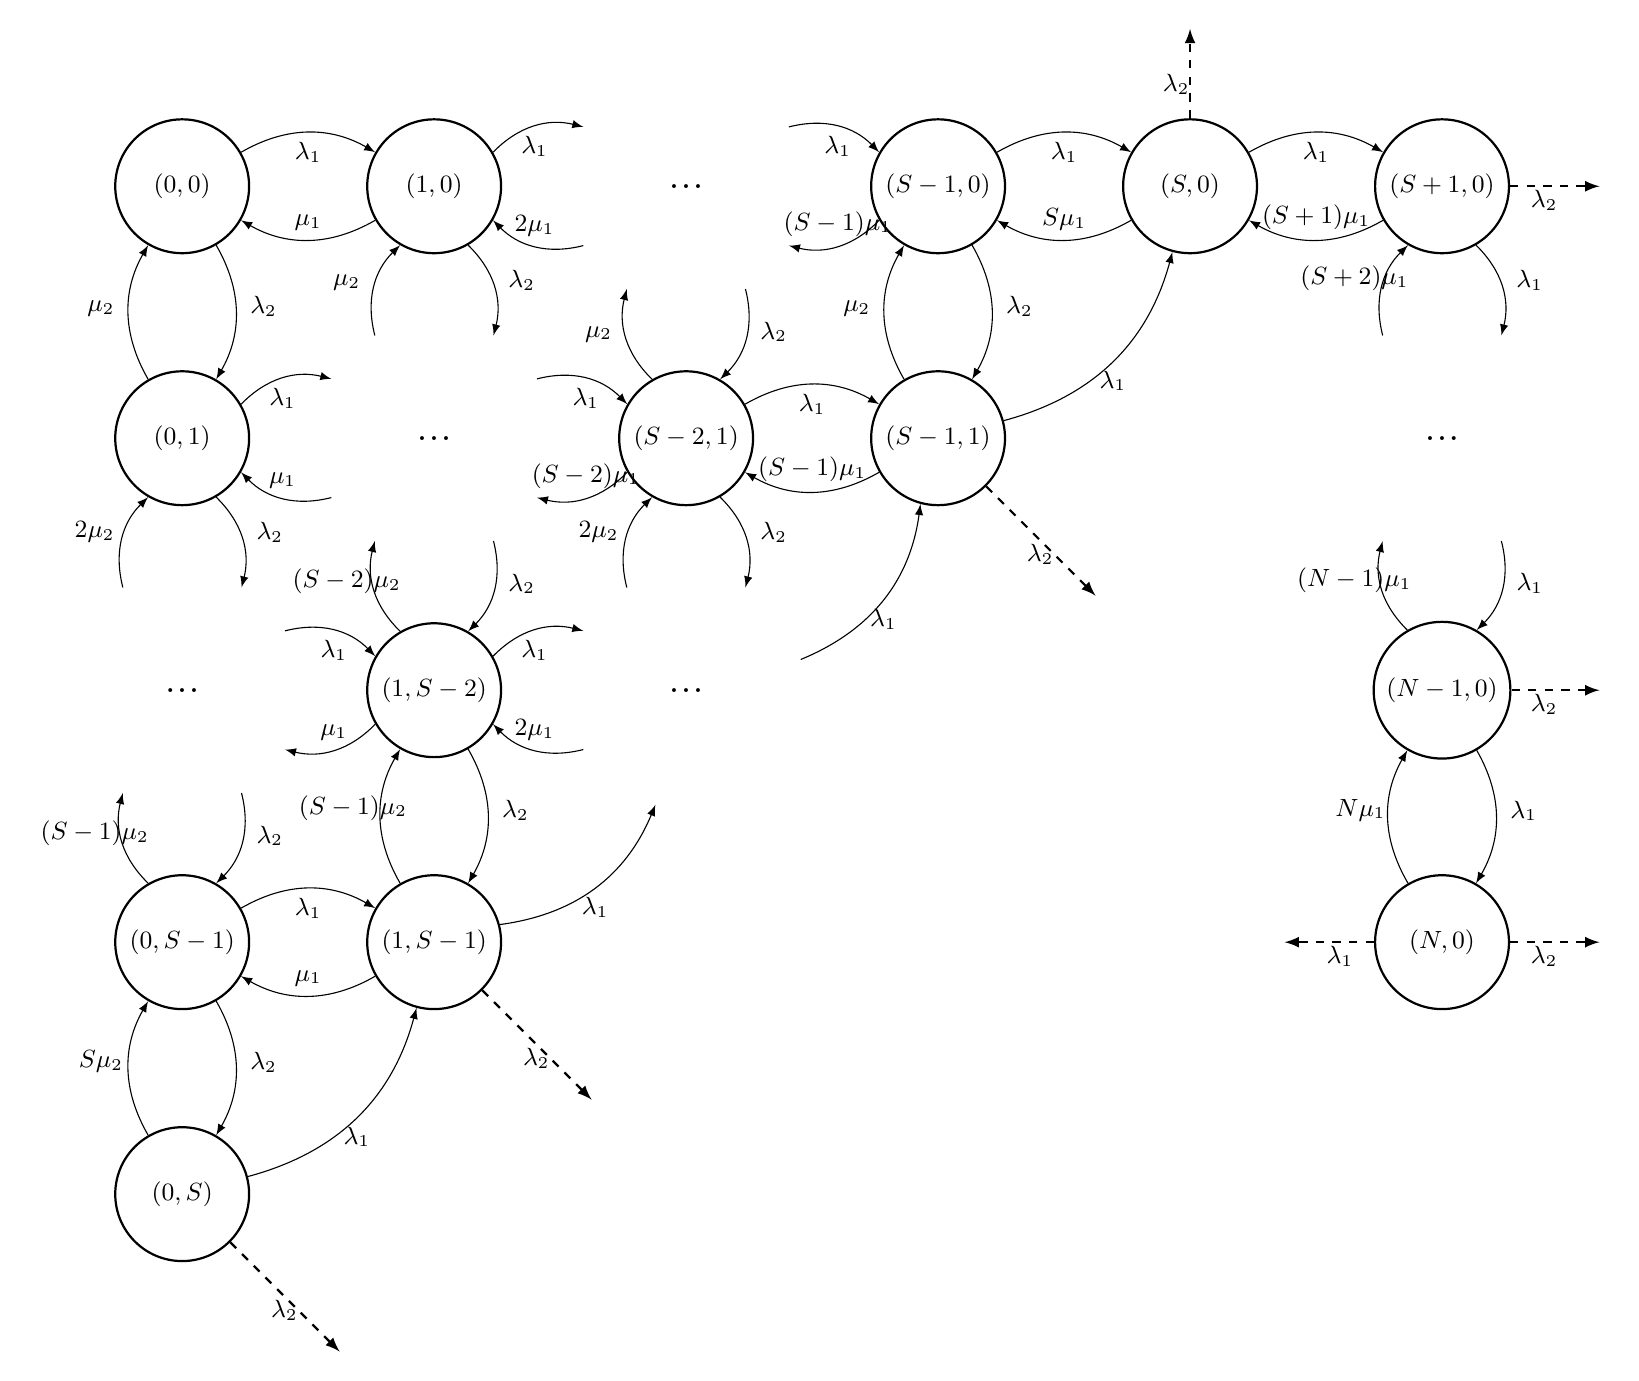
\begin{tikzpicture}[->,node distance=3.2cm,>=latex,font=\small, minimum width=1.7cm]

    \tikzstyle{round}=[thick,draw=black,circle]

    \node[round] 			    (00) {$(0,0)$};
    \node[round,right of=00]    (10) {$(1,0)$};
    \node[round,below of=00]    (01) {$(0,1)$};
    
	\node[circle,draw=white,right of=10, minimum width = 3cm]    (B0) {\LARGE ...};
    \node[circle,draw=white,below of=01, minimum width = 3cm]    (B1) {\LARGE ...};    
    
   	\node[round,right of=B0]    (S-1/0)  	{$(S-1,0)$};
   	\node[round,right of=S-1/0] (S0)	 	{$(S,0)$};
    \node[round,below of=S-1/0] (S-1/1)     {$(S-1,1)$};
    \node[round,left  of=S-1/1] (S-2/1)	{$(S-2,1)$};
   
    \node[round,below of=B1]    (0/S-1)  	{$(0,S-1)$};
   	\node[round,below of=0/S-1] (0S)	 	{$(0,S)$};
    \node[round,right of=0/S-1] (1/S-1)     {$(1,S-1)$};
    \node[round,above of=1/S-1] (1/S-2)     {$(1,S-2)$};
    
    
    \node[circle,below of=10, minimum width = 3cm]    (B2) {\LARGE ...};
    \node[circle,draw=white,right of=1/S-2, minimum width = 3cm]    (B3) {\LARGE ...};
   
    \node[round,right of=S0] (S+1/0)	 	{$(S+1,0)$};  
    \node[circle,draw=white,below of=S+1/0, minimum width = 3cm]    (B4) {\LARGE ...};
    \node[round,below of=B4] (N-1/0)	 	{$(N-1,0)$};  
    \node[round,below of=N-1/0] (N0)	 	{$(N,0)$};  
   
    \draw[dashed,thick, ->] (N0) -- +(2,0) node[xshift=-20,yshift=-5]  {$\lambda_2$};
    \draw[dashed,thick, ->] (N0) -- +(-2,0) node[xshift=20,yshift=-5]  {$\lambda_1$};
    
    \draw[dashed,thick, ->] (N-1/0) -- +(2,0) node[xshift=-20,yshift=-5]  {$\lambda_2$};
    \draw[dashed,thick, ->] (S+1/0) -- +(2,0) node[xshift=-20,yshift=-5]  {$\lambda_2$};
    \draw[dashed,thick, ->] (S0) -- +(0,2) node[xshift=-5,yshift=-20]  {$\lambda_2$};
    \draw[dashed,thick, ->] (1/S-1) -- +(2,-2) node[xshift=-20,yshift=15]  {$\lambda_2$};
    \draw[dashed,thick, ->] (S-1/1) -- +(2,-2) node[xshift=-20,yshift=15]  {$\lambda_2$};
    \draw[dashed,thick, ->] (0S) -- +(2,-2) node[xshift=-20,yshift=15]  {$\lambda_2$};
   
 	\path 
 	
 	(S+1/0)edge[bend left,above]    node {$(S+1)\mu_1$} 		(S0)
 		   edge[bend left,above]       node [xshift=10,yshift=-5]  {$\lambda_1$} 		(B4)
 	
 	(B4)   edge[bend left,above]       node [xshift=-10,yshift=-5] {$(S+2)\mu_1$} 		(S+1/0)
 		   edge[bend left,above]       node [xshift=10,yshift=-5]  {$\lambda_1$} 		(N-1/0)
 		   
 		   
 	(N-1/0)	 edge[bend left,above]       node [xshift=10,yshift=-5]  {$\lambda_1$} 		(N0)
 			 edge[bend left,above]       node [xshift=-10,yshift=-5] {$(N-1)\mu_1$} 	(B4)
 		   
    (N0) edge[bend left,above]       node [xshift=-10,yshift=-5] {$N\mu_1$} 		(N-1/0)
 	
 	(00) 	edge[bend left,below]		node 					    {$\lambda_1$}		(10)
 		 	edge[bend left,above]       node [xshift=10,yshift=-5]  {$\lambda_2$} 		(01)
 	
 	(10) 	edge[bend left,above]       node 						{$\mu_1$} 			(00)
 		 	edge[bend left,below]		node 					    {$\lambda_1$}		(B0)
 		 	edge[bend left,above]       node [xshift=10,yshift=-5]  {$\lambda_2$} 		(B2)
 	
    (01) 	edge[bend left,above]       node [xshift=-10,yshift=-5] {$\mu_2$} 			(00)
   		 	edge[bend left,below]		node 					    {$\lambda_1$}		(B2)
   	     	edge[bend left,above]       node [xshift=10,yshift=-5]  {$\lambda_2$} 		(B1)
   
    (B0) 	edge[bend left,above]       node 						{$2\mu_1$} 			(10)
    		edge[bend left,above]       node [xshift=10,yshift=-5]  {$\lambda_2$} 		(S-2/1)
    		edge[bend left,below]		node 					    {$\lambda_1$}		(S-1/0)
   		    
    (B1) 	edge[bend left,above]       node [xshift=-10,yshift=-5] {$2\mu_2$} 			(01)
   			edge[bend left,above]       node [xshift=10,yshift=-5]  {$\lambda_2$} 		(0/S-1)
   			edge[bend left,below]		node 					    {$\lambda_1$}		(1/S-2)
   			
   
    (B2) 	edge[bend left,above]       node [xshift=-10,yshift=-5] {$\mu_2$} 			(10)
   		 	edge[bend left,above]       node 						{$\mu_1$} 			(01)
   		 	edge[bend left,above]       node [xshift=10,yshift=-5]  {$\lambda_2$} 		(1/S-2)
   		 	edge[bend left,below]		node 					    {$\lambda_1$}		(S-2/1)
   		 	
    (B3)    edge[bend left,above]       node [xshift=-10,yshift=-5] {$2\mu_2$} 			(S-2/1)
   		    edge[bend left,above]       node 						{$2\mu_1$} 			(1/S-2)   	
   		    edge[bend right,below]		node 					    {$\lambda_1$}		(S-1/1)	 	
   		 	
    (S0) 	edge[bend left,above]       node 						{$S\mu_1$} 			(S-1/0)
 			 edge[bend left,below]		node 					    {$\lambda_1$}		(S+1/0)	
 			 
   	(S-1/0) edge[bend left,below]		node 					    {$\lambda_1$}		(S0)
   			edge[bend left,above]       node [xshift=10,yshift=-5]  {$\lambda_2$} 		(S-1/1)
   			edge[bend left,above]       node 						{$(S-1)\mu_1$} 		(B0)
   
    (S-1/1) edge[bend left,above]       node [xshift=-10,yshift=-5] {$\mu_2$} 			(S-1/0)
    		edge[bend left,above]       node 						{$(S-1)\mu_1$} 		(S-2/1)
    		edge[bend right,below]		node 					    {$\lambda_1$}		(S0)	 
    
    (S-2/1) edge[bend left,below]		node 					    {$\lambda_1$}		(S-1/1)
    		edge[bend left,above]       node [xshift=-10,yshift=-5] {$\mu_2$} 			(B0)
    		edge[bend left,above]       node 						{$(S-2)\mu_1$} 		(B2)
    		edge[bend left,above]       node [xshift=10,yshift=-5]  {$\lambda_2$} 		(B3)
		 
    (0S) 	edge[bend left,above]       node [xshift=-10,yshift=-5]	{$S\mu_2$} 			(0/S-1)
    		edge[bend right,below]		node 					    {$\lambda_1$}		(1/S-1)
   
   	(0/S-1) edge[bend left,below]		node 					    {$\lambda_1$}		(1/S-1)
   			edge[bend left,above]       node [xshift=10,yshift=-5]  {$\lambda_2$} 		(0S)
   			edge[bend left,above]       node [xshift=-10,yshift=-5]	{$(S-1)\mu_2$} 		(B1)
   
    (1/S-1) edge[bend left,above]       node 						{$\mu_1$}  			(0/S-1)
    	    edge[bend left,above]       node [xshift=-10,yshift=-5]	{$(S-1)\mu_2$} 		(1/S-2)
    	    edge[bend right,below]		node 					    {$\lambda_1$}		(B3)
    
    (1/S-2) edge[bend left,above]       node 						{$\mu_1$}  			(B1)
    		edge[bend left,above]       node [xshift=10,yshift=-5]  {$\lambda_2$} 		(1/S-1)
    		edge[bend left,above]       node [xshift=-10,yshift=-5]	{$(S-2)\mu_2$} 		(B2)
    		edge[bend left,below]		node 					    {$\lambda_1$}		(B3)
  
    		
   ;
  
\end{tikzpicture}
\end{adjustbox}
\end{figure}

\begin{adjustbox}{center=\textwidth}
\label{equation:AccessControlAlgorithm1-BalanceEquations}

$\begin{cases} 
(\lambda_1 + \lambda_2)\pi_{(0,0)} = \mu_1\pi_{(1,0)} + \mu_2\pi_{(0,1)} \\

(\lambda_1 + \lambda_2 + i\mu_1)\pi_{(i,0)} = \lambda_1\pi_{(i-1,0)} + \mu_1(i+1)\pi_{(i+1,0)} + \mu_2\pi_{(i,1)} & \forall i \in \mathbb{N} \mid 1 \leq i \leq S-1 \\

(\lambda_1 + \lambda_2 + i\mu_2)\pi_{(0,i)} = \lambda_2\pi_{(0,i-1)} + \mu_1\pi_{(1,i)} + \mu_2(i+1)\pi_{(0,i+1)} & \forall i \in \mathbb{N} \mid 1 \leq i \leq S-1 \\

(S\mu_1+\lambda_1)\pi_{(S,0)} = \lambda_1\pi_{(S-1,0)} + \lambda_1\pi_{(S-1,1)} + (S+1)\mu_1 \pi_{(S+1,0)}\\

(\lambda_1 + S\mu_2) \pi_{(0,S)} = \lambda_2\pi_{(0,S-1)} \\

(i\mu_1 + j\mu_2 + \lambda_1)\pi_{(i,j)} = \lambda_1\pi_{(i-1,j)} + \lambda_2\pi_{(i,j-1)} & \forall i,j \in \mathbb{N} \mid \begin{array} {l} 1 \leq i \leq S-1 \\ 1 \leq j \leq S-1 \end{array} \mid i + j = S \\

(\lambda_1 + \lambda_2 + i\mu_1 + j\mu_2)\pi_{(i,j)} = \lambda_1\pi_{(i-1,j)} + \lambda_2\pi_{(i,j-1)} + \mu_1(i+1)\pi_{(i+1,j)} + \mu_2(j+1)\pi_{(i,j+1)} & \forall i,j \in \mathbb{N} \mid \begin{array} {l} 1 \leq i \leq S-1 \\ 1 \leq j \leq S-1 \end{array} \mid i + j < S \\

(i\mu_1 + \lambda_1)\pi_{(i,0)} = \mu_1(i+1)\pi_{(i+1,0)} + \lambda_1\pi_{(i-1,0)} & \forall i \in \mathbb{N} \mid S+1 \leq i \leq N-1 \\

N\mu_1\pi_{(N,0)} = \lambda_1\pi_{(N-1,0)} \\

\sum \pi_{(i,j)} = 1 & \forall i,j \in \mathbb{N}_0

\end{cases}
$ 
\end{adjustbox}

\subsubsection{Probabilities computing}

although... To properly analyse this system, we need do compute some useful probabilities.

Similarly to the previous case we need to now following probabilities:



\begin{table}[h!]
    \caption{Lista dei file del malware FASTCash}
    \centering
    \small
    \label{tab:MalwareFileList}
     \begin{tabular}{rp{8cm}}

      \toprule

      $\Pi_{\text{SendToCloudlet}}(k)$ & Probability that an arriving job of class $k$ on controller has to be forwarded to cloudlet \\
\\
      $\Pi_{\text{SendToCloud}}(k)$ & Probability that an arriving job of class $k$ on controller has to be forwarded to cloud \\
\\
      $\Pi_{\text{Class2JobInterruption}}(k)$ & Probability that a job of class 2 running on cloudlet has to be interrupted and forwarded to cloud due of  arriving class 1 job on cloudlet. \\

      \bottomrule

    \end{tabular}
\end{table}

Differently from the previous case, owing to the use of a different access control algorithm, jobs of different classes have different probability according to which an arriving job on controller has to be send to cloud. From CTMC analysis, we can easily understand that:


\begin{equation}
\begin{array} {lcl} 
\Pi_{\text{SendToCloud}}(1) & = & P\lbrace{\text{An arrival class 1 job on controller sees $N$ class 1 jobs in cloudlet}}\rbrace \\ 
\\
& = & P\lbrace{n_1 = N}\rbrace \\ 
\\
& = & \pi(N,0)
\end{array}
\end{equation}



\begin{center}
\begin{equation}
\begin{array} {lcl} 
\Pi_{\text{SendToCloud}}(2) & = & P\lbrace{\text{An arrival class 2 job on controller sees that number of jobs in cloudlet exceed or is equal to a given threshold S}}\rbrace \\ 
\\
& = & P\lbrace{n_1 + n_2 \geq N}\rbrace \\ 
\\
& = & \displaystyle \sum_{\substack{n_1,n_2 = 0 \\ n_1 + n_2 = S}}^{S} \pi(n_1,n_2) + \sum_{n_1 = S+1}^{N}\pi(n_1,0) \\
\\
& = & \displaystyle \sum_{\substack{0 \leq n_1 \leq N \\ 0 \leq n_2 \leq S \\ n_1 + n_2 \geq S}} \pi(n_1,n_2)
\end{array}
\end{equation}
\end{center}

\end{document}
